在计算机网络中,速率顾名思义\textbf{是指数据的传输速率},即单位时间内传输的数据量。一般速率有两种描述形式:\textbf{波特率和比特率}。

{\textbf{1. 码元}}

在数字通信中常常用时间间隔相同的符号来表示一个二进制数字,这样的时间间隔内的信号称为二进制码元。

\textbf{{2. 波特率}}

又称为码元传输速率,它\textbf{表示单位时间内数字通信系统所传输的码元个数}(也可以称为\textbf{脉冲个数或者信号变化的次数},对理解某些题有好处,一定记住!),单位是波特(Baud)。1波特表示数字通信系统每秒传输1个码元。码元可以是二进制表示,也可以是多进制表示。

\textbf{{3. 比特率}}

又称为信息传输速率,它\textbf{表示单位时间内数字通信系统所传输的二进制码元个数},即比特数,单位为bit/s。

\textbf{{4. 比特率与波特率的关系}}

正常情况下,\textbf{每比特只能表示两种信号变化(0或1),可看成二进制。}此时每个码元只能携带1bit的信息,所以在数量上,波特率就和比特率相等了。因此,在二进制码元的情况下,比特率在数量上和波特率是相等的。但是,一个码元仅携带一个比特,数据率很低,所以编码专家想办法让一个码元携带更多的比特,以此来提高传输速率,即通过一些手段将信号的变化次数增加,从而让一个码元携带更多的比特,例如,增加到16种信号变化(可以看成十六进制),那么自然就需要4bit(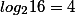
\includegraphics[width=0.78125in,height=0.15625in]{texmath/badcf0log2164},记住这个公式!)来表示,此时一个码元携带了4bit,此时的波特率在数量上就是比特率的4倍。\\
